\documentclass[letterpaper]{amsart}
\usepackage{soul}
\usepackage{graphicx,xcolor}
\usepackage{amsmath,amsthm}
\usepackage{amssymb}
\usepackage{float}
\usepackage[hidelinks]{hyperref}
\usepackage{enumerate}
\usepackage{mathrsfs}

\usepackage[english]{babel}

\theoremstyle{plain}

\newtheorem*{theorem*}{Theorem}
\newtheorem{theorem}{Theorem}[section]
\newtheorem{claim}{Claim}[section]
\newtheorem{definition}{Definition}[section]
\newtheorem{lemma}[theorem]{Lemma}
\newtheorem{proposition}[theorem]{Proposition}
\newtheorem{corollary}[theorem]{Corollary}
\newtheorem{conjecture}[theorem]{Conjecture}
\newtheorem*{question*}{Question}
\newtheorem*{questions*}{Questions}
\newtheorem*{remark*}{Remark}

\def\NN{\mathbb{N}}
\def\ZZ{\mathbb{Z}}
\def\RR{\mathbb{R}}
\def\prob{\mathbb{P}}
\def\esp{\mathbb{E}}
\def\ag{\mathcal{A}}
\def\bg{\mathcal{B}}
\def\CC{\mathcal{C}}
\def\cg{\mathcal{C}}
\def\FF{\mathcal{F}}
\def\dens{\operatorname{dens}}

\newcommand{\define}[1]{\emph{#1}}
\newcommand{\cor}[2][]{#2}

%TIKZ
\usepackage{tikz}
\usetikzlibrary{patterns,positioning,arrows,decorations.markings,calc,decorations.pathmorphing,decorations.pathreplacing}
%\usetikzlibrary{lindenmayersystems}
%\usetikzlibrary{arrows}
%\usepackage{tikz-3dplot}

%\pgfdeclarelindenmayersystem{cayleyPSL2Z}{
%	\rule{A -> [FB+FF[+A]----FF[+A]----FF]++++++}
%	\rule{B -> FBB}}

% %Colors :
% 
%\definecolor{vert}{RGB}{0,178,102}


\title{Title of the paper}
\date{}
\author{Eduardo Silva \\
	\texttt{esilva@dim.uchile.cl}}



\begin{document}
	
	\maketitle 
	
	\begin{abstract}
	abstract
	\end{abstract}	
	
	\textbf{Keywords:} Keyword 1, Keyword 2, Keyword 3.
	
	%%%%%%%%%%%%%%%%%%%%%%
	%%%%%%%%%%%%%%%%%%%%%%
	\section*{Introduction}
	\label{section.introduction}
	
	Introduction.
	
	We show:
	
	{
		\renewcommand{\thetheorem}{\ref{theorem.free_subflow}}
		\begin{theorem}
			Every countable group $G$ has a non-empty, strongly aperiodic subshift on the alphabet $\{0,1\}$.
		\end{theorem}
		\addtocounter{theorem}{-1}
	}
	
	
	{
		\renewcommand{\thetheorem}{\ref{theorem.strongly_aperiodic1}}
		\begin{theorem}
			Every finitely generated group $G$ has a non-empty $G$-effectively closed strongly aperiodic subshift.
		\end{theorem}
		\addtocounter{theorem}{-1}
	}	
	
	
	\section{Preliminaries}
	\label{section.preliminaries}
	
	Throughout this article the groups $G$ considered will \cor[be either countable or finitely generated]{always be countable}; we denote their identity element $1_G$. When $G$ is finitely generated we associate a finite set $S\subset G$ of generators and the undirected right Cayley graph $\Gamma(G,S) = (G, \{ \{g,gs\} \mid g \in G, s\in S\})$ so that $(G,d)$ is a metric space where $d$ is the distance induced on $G$ by $\Gamma(G,S)$. \cor{If two words $w_1,w_2$ in $S^*$ represent the same element in $G$, we write $w_1 =_G w_2$.} We shall denote by $B(g,n) = \{h \in G \mid d(g,h) \leq n\}$ the ball of size $n$ centered in $g \in G$. In general we denote $B_{\Gamma}(v,n)$ the ball of size $n$ centered in $v$ of an arbitrary graph $\Gamma$. \cor{For $g\in G$, we denote by $|g|$ the length of a shortest path from $1_G$ to $g$ in $\Gamma(G,S)$, that is to say $|g|=d(1_G,g)$.} We also denote by $\texttt{WP}(G) := \{ w \in (S\cup S^{-1})^{*} \mid w =_G 1_G \}$ the set of words which can be written using elements 
	from $S$ and their inverses which are equal to $1_G$ in the group $G$. If $\texttt{WP}(G)$ is a decidable language we say that $G$ has decidable word problem. For more references see~\cite{MagnusKarassSolitar2004}.
	
	
	We now give some basic definitions of symbolic dynamics. For a more complete introduction the reader may refer to~\cite{lind1995introduction,ceccherini-SilbersteinC09}. Let $\ag$ be a finite alphabet and $G$ a countable group. The set $\ag^G = \{ x: G \to \ag\}$ equipped with the left group action $\sigma: G \times \ag^G \to \ag^G$ defined by $(\sigma_g(x))_h = x_{g^{-1}h}$ is the \textit{$G$-fullshift}. The elements $a \in \ag$ and $x \in \ag^G$ are called \define{symbols} and \define{configurations} respectively. By taking the discrete topology on $\ag$ we obtain that the set of configurations $\ag^G$ is compact and metrizable. In the case of a countable group, given an enumeration $1_G = g_0,g_1,\dots$ of $G$, the topology is generated by the metric $d(x,y) = 2^{-\inf (\{ n \in \NN \mid\ x_{g_n} \neq y_{g_n}  \})}$. If $E$ is a subset of $\ag^G$, we denote by~$\overline{E}$ its topological closure. In the case of a finitely generated group another possibility which is more practical is $\
	\displaystyle{d(x,y) = 2^{-\inf\{|g|\; \mid\; g \in G:\; x_g \neq y_g\}}}$. This topology is generated by a clopen basis given by the \define{cylinders} $[a]_g = \{x \in \ag^G | x_g = a\in \ag\}$. A \emph{support} is a finite subset $F \subset G$. Given a support $F$, a \emph{pattern with support $F$} is an element $p$ of $\ag^F$, i.e. a finite configuration and we write $supp(p) = F$. We also denote the cylinder generated by $p$ centered in $g$ as $[p]_g = \bigcap_{h \in F}[p_h]_{gh}$
	One says that a pattern $p\in \ag^{F}$ \emph{appears} in a configuration $x \in \ag^G$ if there exists $g \in G$ such that for any $h \in F$, $x_{gh} = p_h$, said otherwise, if there exists $g$ such that $x \in [p]_g$. In this case we write $p \sqsubset x$. We denote the set of finite patterns over $G$ as $\ag_G^* := \bigcup_{F \subset G, |F| < \infty}{\ag^F}$.
	\begin{definition}
		A subset $X$ of $\ag^G$ is a \define{$G$-subshift} if it is $\sigma$-invariant -- $\sigma(X)\subset X$ -- and closed for the cylinder topology. Equivalently, $X$ is a $G$-subshift if and only if there exists a set of forbidden patterns $\FF \subset \ag_G^*$ that defines it.
		$$X=X_\FF := \left\{\ x\in \ag^G\mid \forall p \in \FF, p \not\sqsubset x \right\} = \bigcap_{p \in \FF, g \in G}{\ag^G \setminus [p]_g}.$$
	\end{definition}
	
	That is, a $G$-subshift is a shift-invariant subset of $\ag^G$ which can be written as the complement of a union of cylinders.
	If \cor[the context is clear enough]{it is clear from the context}, we will drop the $G$ and simply refer to a subshift. A subshift $X\subseteq \ag^G$ is \define{of finite type} -- $G$-SFT for short -- if there exists a finite set of forbidden patterns $\FF$ such that $X=X_\FF$. 
	
	Consider a group which is generated by a finite set $S$. A \define{pattern coding} $c$ is a finite set of tuples $c=(w_i,a_i)_{1 \leq i \leq n}$ where $w_i \in (S \cup S^{-1})^{*}$ and $a_i \in \ag$. We say that a pattern coding is \define{consistent} if for every pair of tuples such that $w_i =_G w_j$ ($w_i$ and $w_j$ represent the same element under $G$) then $a_i = a_j$. We say a consistent pattern coding $c$ \define{codifies} a pattern $P$ if every $w_i$ represents an element of $supp(P)$ and for every $g \in supp(P)$ there exists a tuple $(w_i,a_i) \in c$ such that $g =_G w_i$ and $P_g = a_i$.
	
	\begin{definition}
		For a finitely generated group $G$ we say a subshift $X\subseteq \ag^G$ is \define{$G$-effectively closed} if there exists a Turing machine with oracle $\texttt{WP}(G)$ which recognizes a set of pattern codings such that the consistent ones codify a set of patterns $\FF$ such that $X=X_\FF$. If the same property is valid without the oracle we say $X$ is \define{effectively closed}.
	\end{definition}
	
	Being $G$-effectively closed is a generalization of the same concept for $\ZZ$-subshifts where the set of forbidden patterns is a recursively enumerable set of words. 
	
	%	It is also equivalent to a more natural definition of recognizability where instead of using a Turing machine with oracle $\texttt{WP}(G)$ it uses a modified Turing machine -- $G$-Machine -- which has the group $G$ as the tape and moves on the tape by using the generators and their inverses. A more throughout discussion of these concepts and their relations to the classical definition can be found in \cite{ABS2014}.
	
	Let $x\in \ag^G$ be a configuration. The \define{orbit} of $x$ is the set of configurations $orb_\sigma(x)=\left\{\sigma_g(x)\mid g\in G \right\}$, and the \define{stabilizer} of $x$ is the set of group elements $stab_\sigma(x)=\left\{\ g\in G\mid \sigma_g(x)=x\right\}$. \cor[In the context of subshifts, the stabilizer is a normal subgroup of $G$.]{}
	
	\begin{definition}
		A $G$-subshift $X\subseteq \ag^G$ is \define{weakly aperiodic} if for every configuration $x\in X$, $|orb_\sigma(x)|=\infty$. A $G$-subshift $X\subseteq \ag^G$ is \define{strongly aperiodic} if for every configuration $x\in X$, $stab_\sigma(x)=\left\{ 1_G\right\}$.
	\end{definition}
	
	For infinite groups the weak concept of aperiodicity is relevant and implied by strong aperiodicity.
	
	%%%%%%%%%%%%%%%%%%%%%%%
	
	\section{Non-empty strongly aperiodic subshifts}
	\label{section.strongly_aperiodic_subshifts}
	

	
	\subsection{A non-empty strongly aperiodic subshift over $\{0,1\}$ in any countable group.}
	\label{subsection.simpler_proof}
	

	\subsection{A graph-oriented construction and some computational properties}
	\label{subsection.strongly_aperiodic_subshifts_LLL}
	

we still don't know if this kind of construction is always possible. To our knowledge the following question remains open:
	\begin{question*}
	dssad?
	\end{question*}
	
	
	\textbf{Acknoledgements}: This work was partially supported by .
	
	%%%%%%%%%%%%%%%%%%%%%%%
	%%%%%%%%%%%%%%%%%%%%%%%
	\bibliographystyle{plain}
	\begin{thebibliography}{10}
		
		\bibitem[1]{ABS2014}
		Nathalie Aubrun, Sebasti\'an Barbieri, and Mathieu Sablik.
		\newblock A notion of effectiveness for subshifts on finitely generated groups.
		\newblock \cor{{\em Theoretical Computer Science}, 661:35--55, 2017.}
		
		\bibitem[2]{alonetal_nonrepetitivecoloringofgraphs}
		Noga Alon, Jaroslaw Grytczuk, Mariusz Haluszczak, and Oliver Riordan.
		\newblock Nonrepetitive colorings of graphs.
		\newblock {\em Random Structures \& Algorithms}, 21(3-4):336--346, 2002.
		
		\bibitem[3]{AlonSpencer2008}
		Noga Alon and Joel~H. Spencer.
		\newblock {\em The probabilistic method}.
		\newblock Wiley, 2008.
		
		\bibitem[4]{BallierStein2013}
		Alexis Ballier and Maya Stein.
		\newblock The domino problem on groups of polynomial growth.
		\newblock {\em arXiv preprint arXiv:1311.4222}, 2013.
		
		\bibitem[5]{BertheVuillon2000}
		Val\'erie Berth\'e and Laurent Vuillon.
		\newblock Tilings and rotations on the torus: a two-dimensional generalization
		of sturmian sequences.
		\newblock {\em Discrete Mathematics}, 223(1-3):27--53, 2000.
		
		\bibitem[6]{Cohen}
		David~B. Cohen.
		\newblock The large scale geometry of strongly aperiodic subshifts of finite
		type.
		\newblock \cor{{\em Advances in Mathematics}, 308:599--626, 2017.}
		
		\bibitem[7]{CarrollPenland}
		David Carroll and Andrew Penland.
		\newblock {Periodic points on shifts of finite type and commensurability
			invariants of groups.}
		\newblock \cor{{\em New York Journal of Mathematics}, 21:811--822, 2015.}
		
		\bibitem[8]{ceccherini-SilbersteinC09}
		Tullio Ceccherini-Silberstein and Michel Coornaert.
		\newblock {\em Cellular Automata and Groups.}
		\newblock Springer, 2009.
		
		\bibitem[9]{Fernique2006}
		Thomas Fernique.
		\newblock {Multidimensional Sturmian Sequences and Generalized Substitutions}.
		\newblock {\em {International Journal of Foundations of Computer Science}},
		17:575--600, 2006.
		
		\bibitem[10]{gao2009}
		Su~Gao, Steve Jackson, and Brandon Seward.
		\newblock A coloring property for countable groups.
		\newblock {\em Mathematical Proceedings of the Cambridge Philosophical
			Society}, 147:579--592, 11 2009.
		
		\bibitem[11]{glasner2009}
		Eli Glasner and Vladimir~V. Uspenskij.
		\newblock Effective minimal subflows of bernoulli flows.
		\newblock {\em Proc. Am. Math. Soc.}, 137(9):3147--3154, 2009.
		
		\bibitem[12]{MorseHedlund1938}
		Gustav Hedlund and Marston Morse.
		\newblock Symbolic dynamics.
		\newblock {\em American Journal of Mathematics}, 60(4):815--866, 1938.
		
		\bibitem[13]{Hochman2009b}
		Mike Hochman.
		\newblock On the dynamics and recursive properties of multidimensional symbolic
		systems.
		\newblock {\em Inventiones Mathematicae}, 176(1):131--167, 2009.
		
		\bibitem[14]{Jeandel2015}
		Emmanuel Jeandel.
		\newblock Some notes about subshifts on groups.
		\newblock {\em arXiv preprint arXiv:1501.06831}, 2015.
		
		\bibitem[15]{lind1995introduction}
		Douglas~A. Lind and Brian Marcus.
		\newblock {\em An Introduction to Symbolic Dynamics and Coding}.
		\newblock Cambridge University Press, 1995.
		
		\bibitem[16]{Lothaire}
		M.~{Lothaire}.
		\newblock {\em {Algebraic combinatorics on words.}}
		\newblock Cambridge: Cambridge University Press, 2002.
		
		\bibitem[17]{MagnusKarassSolitar2004}
		Wilhelm Magnus, Abraham Karrass, and Donald Solitar.
		\newblock {\em Combinatorial Group Theory: Presentations of Groups in Terms of
			Generators and Relations}.
		\newblock Dover Books on Mathematics Series. Dover Publications, 2004.
		
		\bibitem[18]{fogg2002substitutions}
		N.~Pytheas~Fogg.
		\newblock {\em Substitutions in Dynamics, Arithmetics and Combinatorics},
		volume 1794 of {\em Lecture Notes in Mathematics}.
		\newblock Springer, 2002.
		
		\bibitem[19]{Piantadosi2006}
		Steven~T. Piantadosi.
		\newblock {Symbolic dynamics on free groups.}
		\newblock Master's thesis, {University of North Carolina, Chapel Hill}, 2006.
		
		\bibitem[20]{Piantadosi2008}
		Steven~T. Piantadosi.
		\newblock Symbolic dynamics on free groups.
		\newblock {\em Discrete and Continuous Dynamical Systems}, 20(3):725--738,
		2008.
		
		\bibitem[21]{PavlovSchraudner2009}
		Ronnie Pavlov and Michael Schraudner.
		\newblock Classification of sofic projective subdynamics of multidimensional
		shifts of finite type.
		\newblock {\em Transactions of the American Mathematical Society}, 367(5),
		2014.
		
		\bibitem[22]{pollicott1998dynamical}
		Mark Pollicott and Michiko Yuri.
		\newblock {\em Dynamical Systems and Ergodic Theory}.
		\newblock London Mathematical Society Student Texts. Cambridge University
		Press, 1998.
		
	\end{thebibliography}
	
	
	
\end{document}
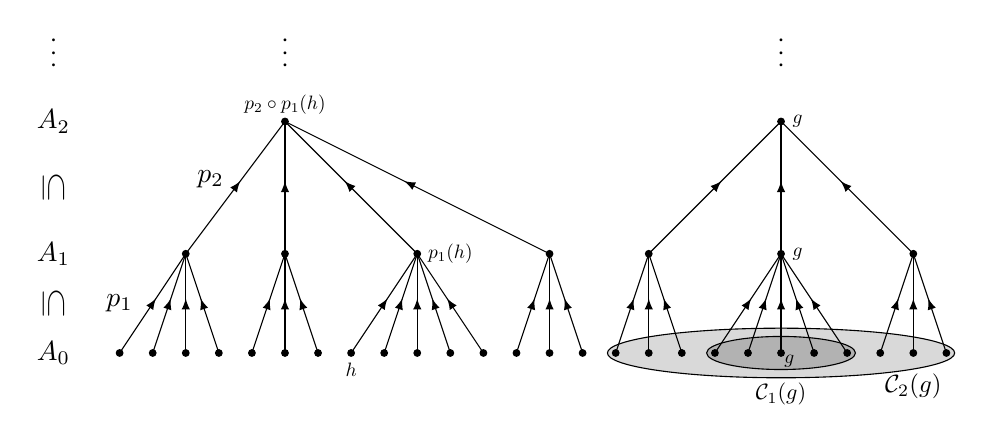
\begin{tikzpicture}[scale=0.42]

%clusters of g
\draw[fill=black!15] (21,0) ellipse (5.25 and 0.75);
\draw[fill=black!30] (21,0) ellipse (2.25 and 0.5);

\draw (21.25,-0.25) node{\scalebox{0.7}{$g$}};
\draw (21.5,3) node{\scalebox{0.7}{$g$}};
\draw (21.5,7) node{\scalebox{0.7}{$g$}};

\draw (8,-0.5) node{\scalebox{0.7}{$h$}};
\draw (11,3) node{\scalebox{0.7}{$p_1(h)$}};
\draw (6,7.5) node{\scalebox{0.7}{$p_2\circ p_1(h)$}};

\draw (21,-1.25) node{\scalebox{0.8}{$\CC_{1}(g)$}};
\draw (25,-1) node{\scalebox{0.9}{$\CC_{2}(g)$}};

% A_0
\foreach \x in {1,...,26}{
	\draw[fill=black] (\x,0) circle (0.1);
}
\draw (-1,0) node{$A_0$};
%\draw (28,0) node{\dots};
\draw (1,1.5) node{$p_1$};

% A_1
\foreach \x in {3,6,10,14,17,21,25}{
	\draw[fill=black] (\x,3) circle (0.1);
}
\draw (-1,1.5) node[yscale=1.5,rotate=-90]{$\subseteq$};
\draw (-1,3) node{$A_1$};
%\draw (28,3) node{\dots};
\draw (3.75,5.25) node{$p_2$};

\foreach \x in {1,...,4}{
	\draw[thin,postaction={decorate,decoration={markings,
			mark=at position .55 with {\arrow[scale=1]{latex}}}}] (\x,0) -> (3,3);
} 
\foreach \x in {5,...,7}{
	\draw[thin,postaction={decorate,decoration={markings,
			mark=at position .55 with {\arrow[scale=1]{latex}}}}] (\x,0) -> (6,3);
}  
\foreach \x in {8,...,12}{
	\draw[thin,postaction={decorate,decoration={markings,
			mark=at position .55 with {\arrow[scale=1]{latex}}}}] (\x,0) -> (10,3);
} 
\foreach \x in {13,...,15}{
	\draw[thin,postaction={decorate,decoration={markings,
			mark=at position .55 with {\arrow[scale=1]{latex}}}}] (\x,0) -> (14,3);
}  
\foreach \x in {16,...,18}{
	\draw[thin,postaction={decorate,decoration={markings,
			mark=at position .55 with {\arrow[scale=1]{latex}}}}] (\x,0) -> (17,3);
} 
\foreach \x in {19,...,23}{
	\draw[thin,postaction={decorate,decoration={markings,
			mark=at position .55 with {\arrow[scale=1]{latex}}}}] (\x,0) -> (21,3);
} 
\foreach \x in {24,...,26}{
	\draw[thin,postaction={decorate,decoration={markings,
			mark=at position .55 with {\arrow[scale=1]{latex}}}}] (\x,0) -> (25,3);
} 

% A_2
\foreach \x in {6,21}{
	\draw[fill=black] (\x,7) circle (0.1);
}
\draw (-1,5) node[yscale=1.5,rotate=-90]{$\subseteq$};
\draw (-1,7) node{$A_2$};
%\draw (28,7) node{\dots};


\foreach \x in {3,6,10,14}{
	\draw[thin,postaction={decorate,decoration={markings,
			mark=at position .55 with {\arrow[scale=1]{latex}}}}] (\x,3) -> (6,7);
} 
\foreach \x in {17,21,25}{
	\draw[thin,postaction={decorate,decoration={markings,
			mark=at position .55 with {\arrow[scale=1]{latex}}}}] (\x,3) -> (21,7);
} 

\draw (-1,9) node[rotate=-90]{$\dots$};
\draw (6,9) node[rotate=-90]{$\dots$};
\draw (21,9) node[rotate=-90]{$\dots$};



\end{tikzpicture}
\begin{tikzpicture}[scale=1]

% \draw[step=0.125,black!15,thin] (-3,-4) grid (3,4); 
% \draw[step=0.25,black!25,thin] (-3,-4) grid (3,4);
% \draw[step=1.0,black!50,thin] (-3,-4) grid (3,4); 
%  
% \draw[color=vert,fill=vert!30,rounded corners=7pt] (0.5,0.6)--(0.75,0)--(0.5,-0.6)--(-2.3,-0.25)--(-2.3,0.25)--cycle;
% \begin{scope}[shift={(-3.125,1.25)},rotate=120,scale=0.3]
% \draw[color=vert,fill=vert!30,rounded corners=2pt] (0.5,0.75)--(0.75,0)--(0.5,-0.75)--(-4.625,-0.25)--(-4.625,0.25)--cycle;
% \end{scope}
% \begin{scope}[shift={(-3.125,-1.25)},rotate=-120,scale=0.3]
% \draw[color=vert,fill=vert!30,rounded corners=2pt] (0.5,0.75)--(0.75,0)--(0.5,-0.75)--(-4.625,-0.25)--(-4.625,0.25)--cycle;
% \end{scope}

\draw []
[l-system={cayleyPSL2Z, step=4pt, angle=30, axiom=[F+FFF[+FA]----FFF[+FA]----FFF]++++++A, order=4}]
lindenmayer system -- cycle;
%LEFT
\draw[fill=vert] (0.15,0) circle (0.05);
\draw[fill=vert] (-1.65,-0.63) circle (0.05);
\draw[fill=vert] (-1.65,0.63) circle (0.05);
\draw[fill=vert] (-2.42,0.63) circle (0.05);
\draw[fill=vert] (-2.5,1.3) circle (0.05);
\draw[fill=vert] (-2.42,-0.9) circle (0.05);
\draw[fill=vert] (-2.5,-0.23) circle (0.05);
\draw[fill=vert] (-1.6,1.6) circle (0.05);
\draw[fill=vert] (-1.1,-1.3) circle (0.05);
\draw[fill=vert] (-1.1,1.3) circle (0.05);
\draw[fill=vert] (-1.6,-1.8) circle (0.05);

%UP
\draw[fill=vert] (1.15,1.6) circle (0.05);
\draw[fill=vert] (0.3,2.22) circle (0.05);
\draw[fill=vert] (-0.22,1.8) circle (0.05);
\draw[fill=vert] (-0.22,2.62) circle (0.05);
\draw[fill=vert] (1,2.9) circle (0.05);
\draw[fill=vert] (1.62,2.9) circle (0.05);
\draw[fill=vert] (2.2,1.6) circle (0.05);
\draw[fill=vert] (2.25,2.25) circle (0.05);
\draw[fill=vert] (2.25,0.65) circle (0.05);
\draw[fill=vert] (2.72,1.97) circle (0.05);
\draw[fill=vert] (2.72,0.92) circle (0.05);

%DOWN
\draw[fill=vert] (1.15,-1.6) circle (0.05);
\draw[fill=vert] (0.3,-2.22) circle (0.05);
\draw[fill=vert] (-0.22,-1.8) circle (0.05);
\draw[fill=vert] (-0.22,-2.62) circle (0.05);
\draw[fill=vert] (1,-2.9) circle (0.05);
\draw[fill=vert] (1.62,-2.9) circle (0.05);
\draw[fill=vert] (2.2,-1.6) circle (0.05);
\draw[fill=vert] (2.25,-2.25) circle (0.05);
\draw[fill=vert] (2.25,-0.65) circle (0.05);
\draw[fill=vert] (2.72,-1.97) circle (0.05);
\draw[fill=vert] (2.72,-0.92) circle (0.05);

\end{tikzpicture}
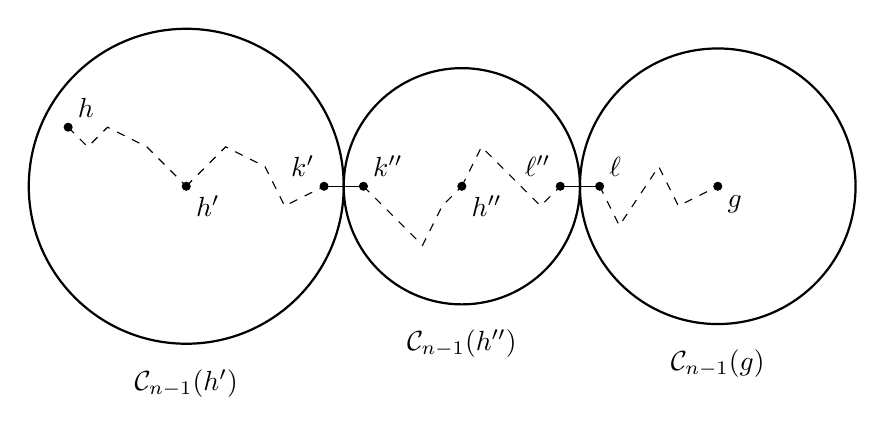
\begin{tikzpicture}[scale=1]


\draw (-1.5,0.75) node[above right]{$h$};
\draw[fill=black] (-1.5,0.75) circle (0.05);

\draw[dashed] (-1.5,0.75) -- (-1.25,0.5) -- (-1,0.75) -- (-0.5,0.5) -- (0,0); 

\draw[thick] (0,0) circle (2); 
\draw (0,0) node[below right]{$h'$};
\draw[fill=black] (0,0) circle (0.05);

\draw (0,-2.5) node[]{$\CC_{n-1}(h')$};

\draw[dashed] (0,0) -- (0.5,0.5) -- (1,0.25) -- (1.25,-0.25) -- (1.75,0);

\draw (1.75,0) node[above left]{$k'$};
\draw[fill=black] (1.75,0) circle (0.05);
%
\draw[] (1.75,0) -- (2.25,0);
%
\draw (2.25,0) node[above right]{$k''$};
\draw[fill=black] (2.25,0) circle (0.05);

\draw[dashed] (2.25,0) -- (2.5,-0.25) -- (3,-0.75) -- (3.25,-0.25) -- (3.5,0);

\draw[thick] (3.5,0) circle (1.5); 
\draw (3.5,0) node[below right]{$h''$};
\draw[fill=black] (3.5,0) circle (0.05);

\draw (3.5,-2) node[]{$\CC_{n-1}(h'')$};

\draw[dashed] (3.5,0) -- (3.75,0.5) -- (4,0.25) -- (4.5,-0.25) -- (4.75,0);

\begin{scope}[shift={(3,0)}]
\draw (1.75,0) node[above left]{$\ell''$};
\draw[fill=black] (1.75,0) circle (0.05);
%
\draw[] (1.75,0) -- (2.25,0);
%
\draw (2.25,0) node[above right]{$\ell$};
\draw[fill=black] (2.25,0) circle (0.05);
\end{scope}

\draw[dashed] (5.25,0) -- (5.5,-0.5) -- (6,0.25) -- (6.25,-0.25) -- (6.75,0);

\draw[thick] (6.75,0) circle (1.75); 
\draw (6.75,0) node[below right]{$g$};
\draw[fill=black] (6.75,0) circle (0.05);

\draw (6.75,-2.25) node[]{$\CC_{n-1}(g)$};

\end{tikzpicture}